\documentclass{beamer}
\usepackage{inconsolata}
\usepackage{caption}
\usepackage{color}
\usepackage{listings}
\usepackage{subfig}
\usepackage{cooltooltips}
\usepackage{hyperref}
\usepackage{perpage}
\usepackage[normalem]{ulem}
\setbeamertemplate{navigation symbols}{}%remove navigation symbols
\usepackage{listings}
\usepackage{color}
\usepackage{framed}

\definecolor{background}{RGB}{39, 40, 34}
\definecolor{string}{RGB}{230, 219, 116}
\definecolor{comment}{RGB}{117, 113, 94}
\definecolor{normal}{RGB}{248, 248, 242}
\definecolor{identifier}{RGB}{166, 226, 46}



\lstset{
  language=C,               			% choose the language of the code
  alsolanguage=Python,            			% choose the language of the code
  alsolanguage=Java,            			% choose the language of the code
  numbers=none,                   		% where to put the line-numbers
  stepnumber=1,                   		% the step between two line-numbers.        
  numbersep=5pt,                  		% how far the line-numbers are from the code
  extendedchars=true,
  numberstyle=\tiny\color{black}\ttfamily,
  backgroundcolor=\color{background},  		% choose the background color. You must add \usepackage{color}
  showspaces=false,               		% show spaces adding particular underscores
  showstringspaces=false,         		% underline spaces within strings
  showtabs=false,                 		% show tabs within strings adding particular underscores
  frame=single,
  framerule=0pt,
  tabsize=4,                      		% sets default tabsize to 2 spaces
  captionpos=n,                   		% sets the caption-position to bottom
  breaklines=true,                		% sets automatic line breaking
  breakatwhitespace=true,         		% sets if automatic breaks should only happen at whitespace
  title=\lstname,                 		% show the filename of files included with \lstinputlisting;
  basicstyle=\color{normal}\tiny\ttfamily,					% sets font style for the code
  keywordstyle=\color{magenta}\tiny\ttfamily,	% sets color for keywords
  stringstyle=\color{string}\tiny\ttfamily,		% sets color for strings
  commentstyle=\color{comment}\tiny\ttfamily,	% sets color for comments
  emph={True, False, format_string, eff_ana_bf, permute, eff_ana_btr, KeyError,
  ValueError, ZeroDivisionError},
  emphstyle=\color{identifier}\tiny\ttfamily,
  morekeywords={with, as}
}

\lstset{literate=%
   *{0}{{{\color{cyan}0}}}1
    {1}{{{\color{cyan}1}}}1
    {2}{{{\color{cyan}2}}}1
    {3}{{{\color{cyan}3}}}1
    {4}{{{\color{cyan}4}}}1
    {5}{{{\color{cyan}5}}}1
    {6}{{{\color{cyan}6}}}1
    {7}{{{\color{cyan}7}}}1
    {8}{{{\color{cyan}8}}}1
    {9}{{{\color{cyan}9}}}1
}



\newenvironment{enum}{
\begin{enumerate}
  \setlength{\itemsep}{1pt}
  \setlength{\parskip}{0pt}
  \setlength{\parsep}{0pt}
}{\end{enumerate}}

\hypersetup{
  colorlinks=true,
  urlcolor=pink,
}

\MakePerPage{footnote}

\title{Python 101}
\subtitle{Lec04 \\ Useful data structures and modules}
\author{thoum}

\begin{document}
\frame{\titlepage}

\begin{frame}
\frametitle{What have we learned so far?}
  \begin{center}
  
\includegraphics[width=80mm]{../lec04/python_art.png}
  \end{center}
\end{frame}

\begin{frame}
\frametitle{Turing Complete}
  In theory, we \textit{can} do everything\tiny{a computer can} \normalsize with what we have learned so far.
  That does not imply efficiency.
  
\end{frame}

\begin{frame}
  Python provides datatypes and $MANY$ useful modules that will help us.\\
  Today, we will take a peek at some of them.
\end{frame}

\begin{frame}
\frametitle{Container Datatypes}
  Things that holds other things (\textit{e.g.} tuples, lists, etc.).\\
  \bigskip
  So far, we have used lists and tuples to store series of values.\\
  But there are different containers for different times.
\end{frame}

\begin{frame}{Dictionary}
  Similar to a list, but instead of \textit{int} as indices, we can use
  objects that are 
  \href{https://docs.python.org/3.7/glossary.html\#term-hashable}{hashable}
  as indices(a.k.a. key).

  Instead of comparing the key with every key it has, \textit{dictionary}
  usually
  \footnote{\href{https://en.wikipedia.org/wiki/Collision_(computer_science)}{Hash
  Collision}} does it efficiently.
\end{frame}

\begin{frame}{Hashing}
  Mapping data of arbitrary size onto data of a fixed size.

  Mapping words to its first letters, mapping students to student IDs,
  mapping your socks to the colors of white, grey and black to pair them, they are all hashing.
\end{frame}

\begin{frame}{Hashing Example}
  $a=1, b=2, ...\ z=26$\\
  score of a word = $\Sigma value(c_i)\ mod\ 101$
  \begin{lstinputlisting}
    {rough_hash.py}
  \end{lstinputlisting}
\end{frame}

\begin{frame}{Hashing}
  Hashing by itself is an important topic with wide range of usage(Encryption,
  Bitcoins...), but will not go into further details.
\end{frame}

\begin{frame}{Using Dictionaries}
  \begin{lstinputlisting}
    {dict_example.py}
  \end{lstinputlisting}
\end{frame}

\begin{frame}{Using Dictionaries}
  \begin{lstinputlisting}
    {dict_example2.py}
  \end{lstinputlisting}
\end{frame}

\begin{frame}{set}
  Unordered collection of $unique$ hashable objects.\\
\end{frame}

\begin{frame}{set examples}
  removing duplicates
  \begin{lstinputlisting}
    {./set_example.py}
  \end{lstinputlisting}
\end{frame}

\begin{frame}{set examples}
  testing membership\\
  list version: 3.6s, set version: 0.05s
  \begin{lstinputlisting}
    {./set_membership.py}
  \end{lstinputlisting}
\end{frame}

\begin{frame}[fragile]{set examples}
  For other operations like union(), intersection(), difference(), look
  \href{https://docs.python.org/3.7/library/stdtypes.html\#set}{here}.
  Or
  \begin{lstlisting}
dir(set)
  \end{lstlisting}
  to see the methods available.
\end{frame}

\begin{frame}{Counter}
  Counts occurrences
  \begin{lstinputlisting}
    {./counter_example.py}
  \end{lstinputlisting}
  Other operations are on the website.
\end{frame}

\begin{frame}{deque}
  Double Ended Queue

  Use instead of \textit{list} when inserting, popping happens at the beginning
  of the list. \textit{e.g.} keeping track of values for moving average?\\
  Insert, pop at the beginning of the list creates an overhead of
  shifting every other element to the left.\\
\end{frame}

\begin{frame}{deque vs list}
  list:3.920s, deque: 0.015s
  \begin{lstinputlisting}
    {./deque_list.py}
  \end{lstinputlisting}
\end{frame}

\begin{frame}{deque vs list}
  List outperforms deque in random access\\
  list:0.111s, deque: 3.597s
  \begin{lstinputlisting}
    {./deque_access.py}
  \end{lstinputlisting}
\end{frame}

\begin{frame}{What to use?}
  In choosing the right $thing$ to use, having a slight idea of complexity
  would help.
\end{frame}

\begin{frame}{Time/Memory Complexity}
  How long does an operation take? How much memory does it use?\\
\end{frame}

\begin{frame}{Time Complexity}
  When input size is $N$
  Some operation might take constant time. \textit{e.g.} lst[i]

  Some operation might take time proportional to N.

  \textit{e.g.} iterating over a list

  Some operation might take time proportional to $N^{2}$.

  \textit{e.g.} matrix multiplication\\

  Some operation might take time proportional to $Nlog(N)$.

  \textit{e.g.} sorting
\end{frame}

\begin{frame}{Pool}
  Parallel Computing is an advanced topic, as it requires careful coding to
  avoid errors like deadlock. ($e.g.$ dining philosophers)\\
  But, Python's Pool allows us to do simple parallel computing.(use with care)
\end{frame}

\begin{frame}{Pool}
  \begin{lstinputlisting}
    {./pool.py}
  \end{lstinputlisting}
\end{frame}

\begin{frame}[fragile]{Pool}
  The order of execution is not guaranteed, although the end result would be
  ordered.
  \begin{center}
  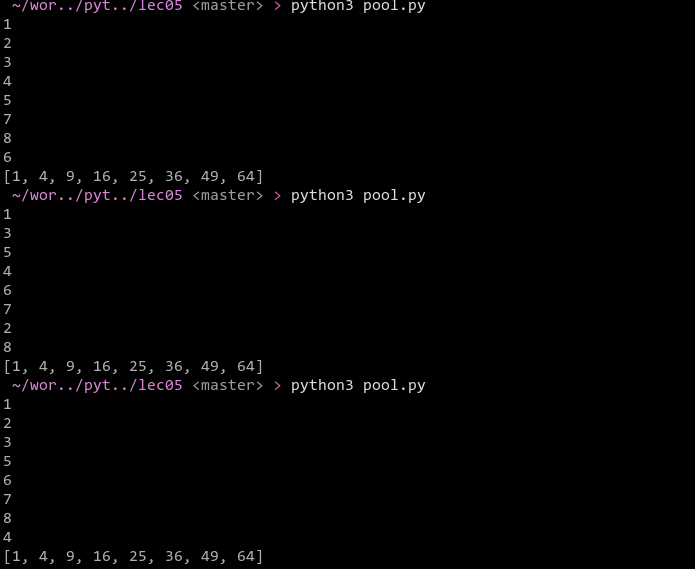
\includegraphics[width=80mm]{./pool_result.png}
  \end{center}
\end{frame}

\begin{frame}{Pool Explained}
  Pool(4) means we will use 4 cpus.\\
  Pool() defaults to $os.cpu\_count()$.(Mine has 4)\\
\end{frame}

\begin{frame}[fragile]{Pool Explained}
 $with$ keyword handles initalization and cleanup of certain operations
\begin{lstlisting}
# p is only effective within the 'with'
with Pool() as p:
    # do something

p = Pool()
# do something
p.close()
p.join()
\end{lstlisting}
\end{frame}

\begin{frame}{Pool Performance}
  \begin{lstinputlisting}
    {./multi_single.py}
  \end{lstinputlisting}
\end{frame}

\end{document}
